%iffalse
\let\negmedspace\undefined
\let\negthickspace\undefined
\documentclass[journal,12pt,onecolumn]{IEEEtran}
\usepackage{cite}
\usepackage{amsmath,amssymb,amsfonts,amsthm}
\usepackage{algorithmic}
\usepackage{multicol}
\usepackage{graphicx}
\usepackage{textcomp}
\usepackage{xcolor}
\usepackage{txfonts}
\usepackage{listings}
\usepackage{enumitem}
\usepackage{mathtools}
\usepackage{gensymb}
\usepackage{comment}
\usepackage[breaklinks=true]{hyperref}
\usepackage{tkz-euclide} 
\usepackage{listings}
\usepackage{gvv}                                        
%\def\inputGnumericTable{}                                 
\usepackage[latin1]{inputenc}                                
\usepackage{color}                                            
\usepackage{array}                                            
\usepackage{longtable}                                       
\usepackage{calc}                                             
\usepackage{multirow}                                         
\usepackage{hhline}                                           
\usepackage{ifthen}                                           
\usepackage{lscape}
\usepackage{tabularx}
\usepackage{array}
\usepackage{float}
\newtheorem{theorem}{Theorem}[section]
\newtheorem{problem}{Problem}
\newtheorem{proposition}{Proposition}[section]
\newtheorem{lemma}{Lemma}[section]
\newtheorem{corollary}[theorem]{Corollary}
\newtheorem{example}{Example}[section]
\newtheorem{definition}[problem]{Definition}
\newcommand{\BEQA}{\begin{eqnarray}}
\newcommand{\EEQA}{\end{eqnarray}}
\newcommand{\define}{\stackrel{\triangle}{=}}
\theoremstyle{remark}
\newtheorem{rem}{Remark}

% Marks the beginning of the document
\begin{document}
\bibliographystyle{IEEEtran}
\vspace{3cm}

\title{\textbf{NCERT 9.4.3}}
\author{EE24BTECH11032- John Bobby}
\maketitle
\bigskip
\textbf{Question:} Find the solution for the differential equation $\frac{dy}{dx}+y=1$ using trapezoidal rule.\\
\textbf{Solution:}\\
\section{Trapezoidal Method }
From the question 
\begin{align}
    \frac{dy}{dx}=1-y
\end{align}
Let
\begin{align}
    f\brak{x,y}=1-y\\
    y\brak{0}=0
\end{align}
From Forward Euler method:
\begin{align}
\frac{y_{n+1}-y_{n}}{h}=f\brak{x_{n},y_{n}}
\end{align}
From Backward Euler method:
\begin{align}
    \frac{y_{n+1}-y_{n}}{h}=f\brak{x_{n+1},y_{n+1}}
\end{align}
On adding both equation \brak{4} and \brak{5}, We get the Trapezoidal Method
\begin{align}
    \frac{y_{n+1}-y_{n}}{h}=\frac{1}{2}\sbrak{f\brak{x_n,y_n}+f\brak{x_{n+1},y_{n+1}}}\\
    y_{n+1}=y_{n}+\frac{h}{2}\sbrak{f\brak{x_n,y_n}+f\brak{x_{n+1},y_{n+1}}}\\
    y_{n+1}=y_n+\frac{h}{2}\sbrak{1-y_n+1-y_{n+1}}=y_n+\frac{h}{2}\sbrak{2-y_n-y_{n+1}}
\end{align}
On rearranging, we get the difference equation
\begin{align}
    y_{n+1}=\frac{2-h}{2+h}y_n+\frac{2h}{2+h}\\ 
    x_{n+1}=x_n +h
\end{align}
\section{Laplace Transform}
Take the Laplace transform of both sides,\\
\begin{align}
    \mathcal{L}\left\{\frac{dy}{dx}\right\} = \mathcal{L}\{1 - y\}
\end{align}
Using the Laplace transform properties,\\
\begin{align}
    \mathcal{L}\left\{\frac{dy}{dx}\right\} = sY(s) - y(0), \quad \mathcal{L}\{1\} = \frac{1}{s}, \quad \mathcal{L}\{y(t)\} = Y(s)
\end{align}
On rearranging,\\
\begin{align}
    sY(s) - y(0) = \frac{1}{s} - Y(s)\\
    sY(s) + Y(s) = \frac{1}{s} + y(0)\\
    Y(s)(s + 1) = \frac{1}{s} + y(0)\\
    Y(s) = \frac{1}{s(s+1)} + \frac{y(0)}{s+1}
\end{align}
Taking the inverse laplace transform \\
\begin{align}
\mathcal{L}^{-1}\brak{Y\brak{s}}=y\brak{x}\\
    \mathcal{L}^{-1}\brak{\frac{1}{s\brak{s+1}}}=1-e^{-x}\\
    \mathcal{L}^{-1}\brak{\frac{y\brak{0}}{s+1}}=y\brak{0}e^{-x}\\
    y\brak{x}=1-e^{-x}+y\brak{0}e^{-x}
\end{align}
As $y\brak{0}=0$
The solution is 
\begin{align}
    y\brak{x}=1-e^{-x}
\end{align}
\section{Bilinear Transform}
Let the laplace transform of $f\brak{x,y}=1-y$ be $X\brak{s}$
\begin{align}
    X\brak{s}=\mathcal{L}\brak{f\brak{x,y}}
\end{align}
Applying laplace transform on both sides of equation 
\begin{align}
    sY\brak{s}=X\brak{s}
\end{align}
Let $H\brak{s}$ be defined such that
\begin{align}
    H\brak{s}=\frac{Y\brak{s}}{X\brak{s}}\\
    H\brak{s}=1/s
\end{align}
Applying bilinear transform which converts s-domain to z-domain
\begin{align}
    s = \frac{2}{h} \brak{\frac{1 - z^{-1}}{1 + z^{-1}}} \\
    H(z) = \frac{h}{2} \brak{\frac{1 + z^{-1}}{1 - z^{-1}}} \\
    Y(z) = \frac{h}{2} \brak{\frac{1 + z^{-1}}{1 - z^{-1}}} X(z) \\
\end{align}
On rearranging,
\begin{align}
    zY\brak{z}-Y\brak{z}=\frac{h}{2}\brak{zX\brak{z}+X\brak{z}}
\end{align}
Applying Z inverse transform,
\begin{align}
    y_{n+1}-y_{n}=\frac{h}{2}\brak{f\brak{x_{n+1},y_{n+1}}+f\brak{x_n,y_n}}\\
    y_{n+1}-y_{n}=\frac{h}{2}\brak{1-y_{n+1}+1-y_n}\\
    y_{n+1}-y_{n}=\frac{h}{2}\brak{2-y_{n+1}-y_n}\\
    y_{n+1}=y_{n}+\frac{h}{2}\brak{2-y_{n+1}-y_n}
\end{align}
Equation $\brak{34}$ is the same difference equation obtained in equation $\brak{8}$


\begin{figure}[h!]
    \centering
    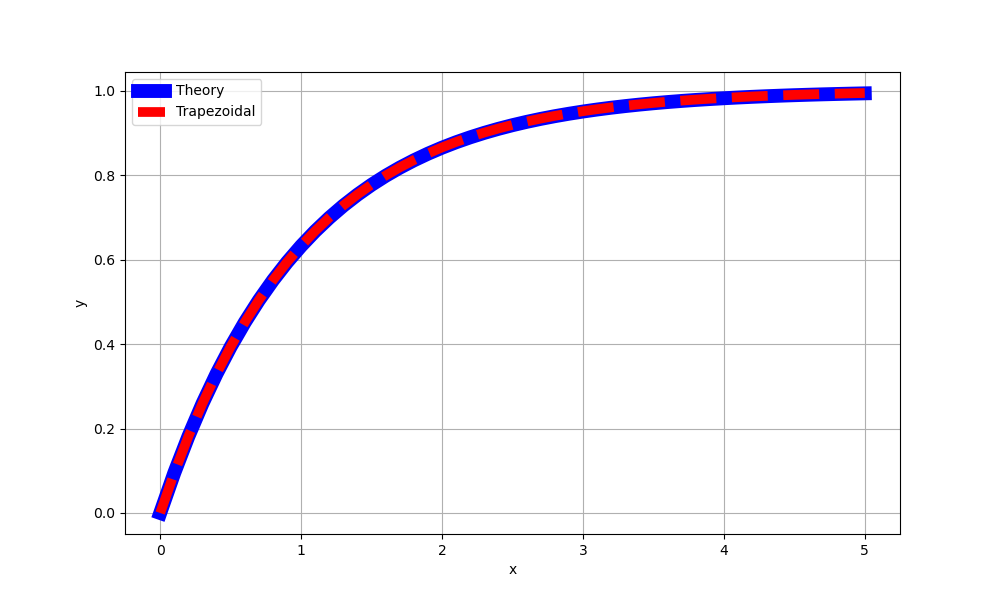
\includegraphics[width=0.7\columnwidth]{figs/Q2.png}
    \label{stemplot}
\end{figure}
\end{document}

